% !TEX root = ./paper.tex

\subsection{\tcpls Transport Services}
\label{sec:transport-services}

%\todo{parler de secure control channel ? (mp): Pour moi non, c'est une vue de
%l'esprit, ça équivaut a dire qu'on peut utiliser des nouveaux records tls}

By leveraging \tcpls records and extensions, we can design new modern transport
services atop the combination of \tcp and \tls. In this subsection, we answer 
our second research question ({\small\textit{RQ2}}) by presenting three 
transport 
services: stream multiplexing (Section~\ref{sec:datastreams}), connection 
migration (Section~\ref{sec:multipath}), and bandwidth aggregation 
(Section~\ref{sec:multipath}). We leverage the \tcpls records
to multiplex concurrent encrypted bytestreams. By extending the \tls handshake, \tcpls allows joining several \tcp connections to a single \tcpls session to support
connection migration, stream steering and %multipath capabilities, mitigating 
%Head-of-Line
%blocking and enabling
bandwidth aggregation.
%aggregation and Head-of-Line blocking resilience.
These features are built atop the TCP bytestream, and as such they avoid 
middleboxes interference that modify the TCP header.

\subsubsection{Stream Multiplexing}\label{sec:datastreams}
%%%%%%%%%%%%%%%%%%%%%%%%%%%%%%%%%

\begin{figure}[!t]
	\centering
	\begin{bytefield}[bitheight=\widthof{aw}]{32}
		\bitbox[]{1}{\small N} & \bitbox[]{9}{} & \bitbox[]{3}{\small N-32} &
		& \bitbox[]{7}{} &
		\bitbox[]{1}{\small 64} & \bitbox[]{9}{} & \bitbox[]{3}{\small 0} \\
		\bitbox{32}{TLS 1.3 AEAD Initial Vector}  \\
		\bitbox[]{12}{+} & \bitbox[]{8}{} & \bitbox[]{12}{$\oplus$} \\
		\bitbox{12}{\tcpls Stream ID} & \bitbox[]{8}{} & \bitbox{12}{Record sequence}
	\end{bytefield}
	\caption{The AEAD Nonce of \tcpls Streams is derived from \tls 1.3.}
	\label{fig:aead-iv}
\end{figure}

Stream Multiplexing is a transport service that has been part of recent
protocols such as \sctp~\cite{rfc4960}, \quic~\cite{rfc9000} and HTTP/2.0
\cite{rfc7540}. The latter also proposes multiplexing with an independent
framing system atop the \tls-encrypted \tcp bytestream. In \tcpls, we choose to
implement multiplexing with \tcpls records. We dedicate a \tcpls record type to
\tcpls stream data. Each stream has a separate cryptographic context allowing
concurrent encryption and decryption of data within the same session.  A \tcpls
stream consists of a sequence of \tcpls stream data records encrypted with their
cryptographic contexts. Each stream is attached to one \tcp connection.

One simple way to provide separate cryptographic contexts is to use multiple
application-level keys. But this is known to degrade the security properties
proportionally to the number of additional keys~\cite{chatterjee2011another}. To
overcome this, we propose an Initial Vector (IV) derivation technique that
enables independent encryption/decryption for each stream without this security
degradation. We add two goals to the design of this technique. First, the 
TLS 1.3 wire format must be preserved to avoid possible middleboxes 
interference. Second, the resulting nonce must be unique for each record of 
each stream in order to maintain the security properties of AEAD.

Figure~\ref{fig:aead-iv} illustrates how the AEAD IV is computed for a given
\tcpls record of a \tcpls stream. First the left-most bits of the IV derived
from the \tls handshake are summed with the 32-bit \tcpls Stream ID. Then the
right-most bits are XORed with the stream 64-bit record sequence number. Each
\tcpls stream has a separate record sequence number space. This combination of
IV manipulation guarantees that the resulting IV is unique for each record of
all \tcpls streams given a unique Stream ID and sequence number. The 
Stream ID space is split between the client
and the server. Stream ID 0 is equivalent to the cryptographic context
derived directly from the handshake.
%\todo{Il faut expliquer comment les stream id sont choisis pour garantir
%l'unicité}

To avoid possible middleboxes interference, in addition to the record sequence
number, the \tcpls Stream ID is kept implicit as well. When an endpoint receives
a \tcpls record, we leverage the AEAD cipher to check the authentication tag
repeatedly until the correct \tcpls Stream ID is found. 
%An optimized implementation would not involve 
It does not involve a complete decryption as all TLS 1.3 AEAD
ciphers use an Encrypt-then-MAC construct~\cite{rfc7366, rfc8446}, and the tag
verification is computationally light, especially on 
AES-GCM~\cite{mcgrew2004galois}. Reducing this cost could be achieved by adding 
explicit signaling when an other stream is scheduled over the \tcp connection\footnote{
The worst case is when the sender schedules records of $N$ streams 
over a \tcp connection. Then,
  \tcpls may announce within the last record of the current stream the Stream 
  ID of the following record.%, thanks to \tcp ordered delivery
%of \tcpls data and control records.
}.
%\todo{citer rfc7366 ? ou les références de ce rfc ?}

From a security standpoint, each failed decryption is considered as a forgery
attempt. However, the limits on confidentiality and integrity for AEAD ciphers
are large before a successful forgery may be considered with non-negligible
probability~\cite{luykx2015limits, aeadlimits}. For example, in the case of
ChaCha20 + Poly1305, an adversary making $2^{60}$ forgery attempts succeeds with
probability $2^{-33}$.
%\todo{Should we mention that one stream cannot be used on two connections at
%the same time?}

%The classical solution to support streams in a transport protocol is to assign
%an identifier to each stream and send the data from stream $x$ as a tuple
%$x,seq,data$ where $seq$ is a sequence number. This is the solution chosen by
%\sctp~\cite{rfc4960} and \quic~\cite{draft-ietf-quic-transport}. \tcpls relies
%on cryptographic properties to support several streams.

%\paragraph*{Cryptographic Details and Tricks} In \tcpls, each stream has its own
%cryptographic context. All streams use the same key but derive a specific
%Initial Vector (IV - also called cryptographic nonce) such that nonce-misuse
%cannot happen. Furthermore, \tcpls derives the IV such that the record sequence
%numbers can securely start at $0$ within each stream.
%
%\tcpls uses only one application-level key for $N$ streams, for each direction.
%We selected this approach to avoid security degradation with the usage of
%multiple keys (by a factor $k$ with $k$ keys)~\cite{chatterjee2011another}.

%To enable all stream sequence numbers to start at 0, we rely on some properties
%of the Authenticated Encryption with Associated Data (AEAD) schemes used by \tls
%1.3. To preserve AEAD security, the AEAD nonce used by \tcpls must be of unique
%use when encrypting and decrypting a record. The initial nonce must also be
%unpredictable for an adversary observing the handshake. \tcpls derives it from
%the \tls handshake session secret in a similar fashion to the \tls
%keys~\cite{rfc8446}. The nonce size ranges from $96$ bits to $128$ bits
%depending on the underlying cipher used. In all cases, for a nonce of size $N$
%bits, \tls computes the cryptographic nonce by concatenating the $N-64$ leftmost
%bits with the 64 lower bits XORed with the record's implicit sequence number
%encoded in 64 bits. XORing the lower 64 bits provides more unpredictability to
%the nonce when the same plaintext is encrypted multiple times with the same
%key~\cite{bellare2016multi,hoang2018multi}. This design implies that we give to
%the underlying cipher the 32 upper bits untouched. The resulting value is then
%concatenated with an internal counter in GCM and used as the blocksize-bits (128
%or 256 bits) stream's counter.
%We observe that the leftmost N-64 bits are available to encode a unique stream number. By
%encoding such a unique number in this part of the cryptographic nonce, we enable
%each stream to start its sequence number at 0 while encrypting its records with
%the same key. This observation means that we can create independent
%cryptographic contexts based on a cryptographic nonce's tweak. This implies
%that stream records can be encrypted and decrypted independently of each other,
%with the same key value. This technique maintains AEAD's core assumption
%(uniqueness of nonce), which means that state of art AEAD's security proof
%starting from that assumption applies to our
%design~\cite{chatterjee2011another} and guarantees the security of our scheme.

%\paragraph*{Carrying Multiple Streams over the Same Transport}
%(mp): TODO Multicore decryption could be listed as an improvement
%Thanks to those separate cryptographic contexts, \tcpls can perform concurrent
%encryption and decryption between streams while maintaining decryption
%correctness and security, and potentially also use this capability to process
%different streams over different CPU cores.
%Finally, when different streams are carried
%over the same \tcp connection, \tcpls does not explicitely know which stream
%a received record belongs to. To retrieve this information,
%we also
%leverage the AEAD cipher and check the incoming record's authentication tag
%until we find the stream that properly verifies this tag. This operation is
%lightweight: it does not require full decryption of the record because the AEAD
%ciphers used by \tls 1.3 do Encrypt then MAC (and MAC then Decrypt).
%Looking for the right stream that succeeds the tag verification needs to be
%performed once each time the application writes to another stream over the same
%\tcp connection.
%
%Note that, security-wise, each failed decryption is considered a
%forgery attempt. However, we have large limits on the confidentiality and
%integrity with all AEAD ciphers~\cite{luykx2015limits, aeadlimits} before a
%successful forgery may be considered as a non-negligible probability. For
%example, in the case of ChaCha20 + Poly1305, an adversary making $2^{60}$ forgery
%attempts succeeds with probability $2^{-33}$.


\subsubsection{Connection Migration}\label{sec:multipath}

\tcpls allows joining several \tcp connections to an existing \tcpls session.
We leverage this mechanism to implement new transport services such as 
connection migration. Compared to the subflow joining mechanism of
\mptcp~\cite{raiciu2012hard,hesmans2015smapp,hesmans2016enhanced}, our design is
more secure. Indeed, \mptcp supports additional subflows by initially exchanging
short keys inside cleartext \tcp \texttt{Options} during the \tcp handshake~\cite{rfc6824, rfc8684}. These keys are then used to authenticate the association of subflows. An attacker having observed the key exchange during the \tcp handshake can associate subflows to an existing \mptcp connection~\cite{rfc6181}.

\begin{figure}[!t]
	\centering
	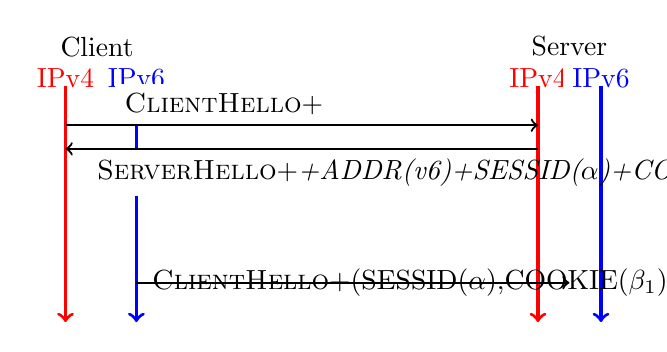
\begin{tikzpicture}
		\colorlet{lightgray}{black!20}
		\tikzstyle{arrow} = [thick,->,>=stealth]
		\tikzset{state/.style={rectangle, dashed, draw, fill=white} }
		\node[black, fill=white] at (0,10) {Client};
		\node[black, fill=white] at (6,10) {Server};
		\node[red, fill=white] at (5.6,9.6) {IPv4};
		\node[blue, fill=white] at (6.4,9.6) {IPv6};
		\node[red, fill=white] at (-0.4,9.6) {IPv4};
		\node[blue, fill=white] at (0.5,9.6) {IPv6};
		\draw[red, very thick,->] (-0.4,9.5) -- (-0.4,6.5);
		\draw[blue, very thick,->] (0.5,9.5) -- (0.5,6.5);
		\draw[red, very thick,->] (5.6,9.5) -- (5.6,6.5);
		\draw[blue, very thick,->] (6.4,9.5) -- (6.4,6.5);
		\draw[black, thick, ->] (-0.4,9) -- (5.6,9) node [midway, fill=white, above,
		text width=4.5cm] {\textsc{ClientHello}+\hello};
		\draw[black, thick, <-] (-0.4,8.7) -- (5.6,8.7) node [pos=0.5, fill=white, below, text width=5.2cm] {\textsc{ServerHello}+\emph{\hello+ADDR(v6)+SESSID($\alpha$)+COOKIE($\beta_1,\beta_2$)}};
		\draw[black, thick, ->] (0.5,7) -- (6.0,7) node [pos=0.4, %fill=white, above,
		text width=4cm] {\textsc{ClientHello}+\join(SESSID($\alpha$),COOKIE($\beta_1$))};
	\end{tikzpicture}
	\caption{\tcpls supports joining additional \tcp
		connections to a \tcpls session. The $SESSID$ and $COOKIE$ in the \textmd{\textsc{ServerHello}} are encrypted with the
		handshake key.}
	\label{fig:join-example}
\end{figure}

\textbf{Joining \tcp connections}. \tcpls leverages \tls
extensions to solve this problem in a more secure manner. 
Figure~\ref{fig:join-example} illustrates the \tls and \tcpls messages 
exchanged when a client connects to a server over IPv4 and later joins another 
connection over IPv6.
First, the client sends a \textsc{ClientHello} containing a \hello. The server 
replies with a \textsc{ServerHello} containing three encrypted extensions. 
First, the server announces its IPv6 address ($ADDR(v6)$). Second, it 
associates one identifier $\alpha$ to the \tcpls session 
(\emph{SESSID($\alpha$)}).
%It uniquely identifies the \tcpls session on the server.
Third, the server provides a list of \tcpls session cookies $\beta_1,\beta_2$ in the \emph{COOKIE} extension. Each of these session cookies enables the client
to join one additional \tcp connection to the \tcpls session. Thus by 
sending $n$ cookies over a session, the server restricts the client to 
join up to $n$ \tcp connections. This prevents resource exhaustion attacks
that are difficult to counter with \mptcp. The server can later send additional
cookies and update its list of addresses.

To join a new \tcp connection to the \tcpls session, for instance over IPv6, the
client sends a \textsc{ClientHello} message containing the session identifier
(SESSID($\alpha$) in Figure~\ref{fig:join-example}) and one of the cookies
provided by the server (COOKIE($\beta_1$) in Figure~\ref{fig:join-example}). The
server uses the session identifier $\alpha$ to find the corresponding \tcpls
session and checks the validity of the cookie. If the \tcpls session and cookie
are valid, the \tcp connection is joined to the \tcpls session. The session
identifier plays the same role as the \mptcp token, but is sent encrypted. The
cookie provides stronger protection than \mptcp's HMAC with security keys
exchanged in cleartext. The \tcpls cookies are sent encrypted by the server and 
can only be used once by the client.
%(i.e.,
%when the server receives a valid cookie, it accepts the connection, attaches it
%to the right \tcpls session, and discards the cookie).


%\tcpls includes a Connection Manager (CM) that controls the underlying \tcp
%connections.
%The CM is fully configurable and exposed to applications through the \tcpls API.
%\tcpls enables the client or the server to associate new \tcp connections to an
%existing \tcpls session. This is similar to \mptcp's path
%managers~\cite{raiciu2012hard,hesmans2015smapp,hesmans2016enhanced},
%but with some differences. First, \tcpls does not suffer from the same
%security limitations as \mptcp. Second, \tcpls supports several multipathing
%modes, including connection failover, bandwidth aggregation and non-aggregated
%multiple paths.

%\paragraph*{1) Better Security Than \mptcp} A \mptcp connection gathers several
%underlying connections called subflows. To ``secure'' the attachment of
%additional subflows, \mptcp hosts exchange short keys in plaintext inside \tcp
%options during the \tcp handshake~\cite{rfc6824, rfc8684}. These keys are then
%used later to authenticate the attachment of subflows. An
%attacker that has observed the initial handshake can attach any subflow to an
%existing \mptcp connection~\cite{rfc6181}. \tcpls leverages its secure channel
%to solves this \texttt{``connection join''} problem in a more secure
%manner. Consider a client connecting to a dual-stack server
%(Figure~\ref{fig:join-example} depicts the \tls messages exchanged in such a
%scenario). The client sends a \textsc{ClientHello} containing the \tls
%extension to negotiate \tcpls. The server replies with a \textsc{ServerHello}
%with three types of encrypted extensions. First, the server announces its IPv4
%and IPv6 addresses. Second, it associates one identifier to the \tcpls session
%(SESSID($\alpha$) in Figure~\ref{fig:join-example}). It uniquely
%identifies the \tcpls session on the server. Third, the server provides a list
%of \tcpls session cookies (COOKIE($\beta_1,\beta_2$) on
%Figure~\ref{fig:join-example}). Each of these session cookies enables the 
%client
%to attach one additional \tcp connection to the \tcpls session. By sending $n$
%cookies, the server indicates that it currently accepts the attachment of only
%$n$ \tcp connections to this session. This prevents resource exhaustion attacks
%that are difficult to counter with \mptcp. The server can send additional
%cookies later and update its list of addresses.
%
%To attach a new connection, e.g., using the server's IPv6 address, the client
%sends a \textsc{ClientHello} message containing the session identifier
%(SESSID($\alpha$) on Figure~\ref{fig:join-example}) and one of the server's
%cookies (COOKIE($\beta_1$) on Figure~\ref{fig:join-example}). The server checks
%the validity of the cookie and then uses the session identifier to attach the
%new \tcp connection to the right \tcpls session. The session identifier and
%cookie play that same role as \mptcp's token. From a security viewpoint, \tcpls'
%session cookie is longer than \mptcp's token. Furthermore, it is sent encrypted
%in the initial \textsc{ServerHello} message, and can only be used once (i.e.,
%when the server receives a valid cookie, it accepts the connection, attaches it
%to the right \tcpls session, and discards the cookie).

\begin{figure}[!t]
	\begin{center}
		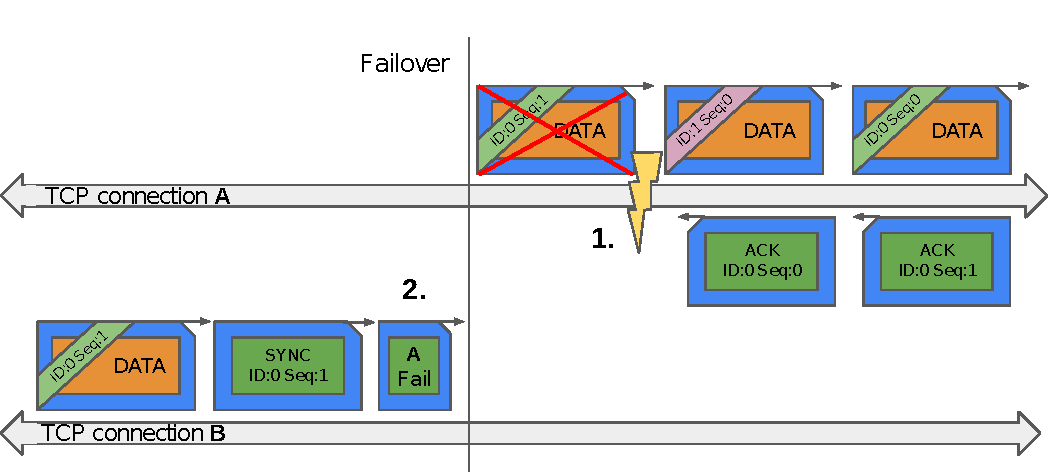
\includegraphics[width=\columnwidth]{figures/tcpls_failover}
	\end{center}
	\caption{Failover resynchronises and retransmits lost \tcpls records 
	from a failed \tcp connection to an other.}
	\label{fig:design-failover}
\end{figure}

\textbf{Failover}.
When a \tcp connection fails, e.g. due to middleboxes or network outages, 
\tcpls leverages its joining mechanism to recover 
the session over another \tcp connection. This is particularly useful on 
multihomed devices that often move out of reach of an given access network, for 
instance a smartphone moving away from a WiFi access point, but also on all 
devices that suffer from middleboxes disrupting TCP connections, for instance a 
firewall introducing TCP RST on idle TCP connections.
Figure~\ref{fig:design-failover} 
illustrates 
how \tcpls reacts to such events during a transfer with two \tcpls streams.
To achieve such a \emph{break-before-make}, 
\tcpls sends acknowledgments for the received records of each stream, allowing
the sender to remove them from its sending buffer.
%Upon reception of Stream-level acknowledgments, the sender can
%manage its sending buffer and remove acknowledged encrypted records.
Looking at \textbf{1.} in Figure~\ref{fig:design-failover}, we can observe that 
three records were sent but only the first two were received and acknowledged 
due to a failure.
Then, looking at \textbf{2.}, the sender notices that the \tcp connection has 
failed and switches to the other one. It explicitly notifies the failure to the 
receiver and synchronizes the transmission sequence using a 
dedicated \tcpls record type (i.e. SYNC in Figure~\ref{fig:design-failover}). 
Then it retransmits the unacknowledged stream data records (i.e. the second 
record of stream 0 in Figure~\ref{fig:design-failover}). 
Explicit synchronization %is required as the \tcpls stream sequence number is 
%implicit and thus 
prevents a lost acknowledgment from desynchronizing the endpoints. 
Notifying the failure to the peer shortens its reaction time.
Thanks to the per-stream cryptographic context, the ciphertext of lost stream 
data records can be retransmitted as is.

%Furthermore,
%the unacknowledged data records sent over the failed \tcp connection are
%transmitted again over a functional one. To resynchronize the session (i.e., 
%the
%implicit encryption/decryption sequence numbers), the
%failover protocol makes the client sends the sequence number of the first 
%record
%within its sending buffer, an $id$ to specify the failed \tcp connection and
%the Stream ID of the stream being moved. This information is encrypted with
%the default context and sent within the new \tcp connection. Receiving this 
%protocol message, the server now knows
%the sequence number to decrypt some record arriving next on the connection that
%read the failover message. Either the server already processed that record, 
%and can safely
%ignore it and increase the sequence number, or the server did not yet seen that
%record, and can decrypt and process it. The same protocol message and 
%operations
%then goes from the server to the client, and the stream is then resyncronized
%over a new \tcp connection. No messages are required to be encrypted twice.
%\tcpls' Failover mode is optional. Both peers need to activate it or
%negotiate the feature throught the Secure Control Channel.
We present in Section~\ref{sec:perf} measurements quantifying the
performance impact of adding \tcpls record-level acknowledgments. We also
present in Section~\ref{sec:eval_failover} an analysis of recovery speeds during
different type of outages.
%We also give a
%trace example involving a file transfer and the failover protocol in
%Appendix~\ref{app:failover}.
%\todo{Let see if we can bring it back in the text later}

\textbf{Application-triggered Connection Migration}. \tcpls also enables the
application to trigger a connection migration, e.g. based on application-level 
metrics qualifying its experience over the current path. For instance, a video 
streaming application could choose to move its connection to another access 
network whenever the obtained bandwidth does not satisfy the video bitrate 
requirements.
%expected to be used
%over
%healthy networks. %and leveraging a transient usage of bandwidth aggregation.
%(mp): I would leave this aside for now, until we explain application streams.
%The decision to migrate from a healthy network to another one is a
%application one.
%(mp): Yet the following meta-info are not described, and again implementation
%-> section
%4
\tcpls enables the exchange of meta-information to help this
decision.
%The TCPLS protocol and implementation's job is to make it quite simple by
%supporting the exchange of interface's related meta-information to help the
%decision
%making and by offering a simple API.
%Essentially, it means that \tcpls provides a simple API that enables an
%application to migrate when it wishes to do so (e.g.,
For instance, an interactive application running on a smartphone could migrate 
from
LTE to Wi-Fi when it senses an increase in delays due to bufferbloat for a
given period of time, or when a mobile client detects its home Wi-Fi and the
user's preference is to move its traffic to the Wi-Fi if detected.
%when the Wi-Fi appears healthy,
%The semantic of
%the application-level connection migration is built from attaching and closing
%streams in the multipath bandwidth aggregation mode.
%The client that wishes to
%carry such a migration first creates a new \tcp connection and joins the \tcpls
%session over this connection.
To achieve it, the client moves all its \tcpls streams to another \tcp
connection.
%(mp): avoid introducing concepts we define later rather than earlier
%can essentially use Stream Streering, i.e., the client
%\textit{composes} with independent
%features offered by \tcpls.
%(mp) -> section 4
%In a client/server implementation using \tcpls, the
%following protocol composition is realised with only 4 API calls (4 lines of
%code).
First, it creates a new \tcp connection and joins it to the
\tcpls
session. Then, %it steers the \tcpls stream abstraction,
it attaches new streams to the new
connection
%using the stream opening protocol
and removes the old ones from the underperforming connection, effectively moving
the application traffic to the new connection.
%(mp): Lets talk of that in the following section rather
%This stream steering
%mechanism may temporally takes advantage of bandwidth aggregation during the
%fraction of seconds required to open the second stream and close the first one.
%These properties are latter demonstrated in Section~\ref{sec:app-migration}.

%by sending one \textsc{Stream\_Attach} message per stream that needs
%to be migrated. At that moment, the client and the server have potentially
%multiple streams opened over the two network paths and can temporally aggregate
%the bandwidth offered by both paths. Then, after having attached
%all its streams to the new path, the migrating host sends a
%\textsc{Stream\_Close} message over the old \tcp connection for all old streams.
%At this point, the migrating host cannot send new stream data anymore over the
%old connection. Once the remote host has received a \textsc{Stream\_Close}
%message over the old \tcp connection, it knows that the connection is not
%available anymore\todo{?}, and can switch to the other connections. It first sends a
%\textsc{Stream\_Close\_Ack} message for each received \textsc{Stream\_Close}.
%The migrating host can close the old connection upon reception of the last
%\textsc{Stream\_Close\_Ack}, indicating that no more data would be received over
%this connection. Note that these messages are \tls records and are thus sent
%securely and reliably.% by the underlying \tcp connection.

This second type of migration does not require application-level
acknowledgments, but it cannot survive from one of the
underlying connections' failure. During such a migration, data may be sent over
two connections, which brings us to explain how multipath is designed.

\subsubsection{Multipath capabilities}

Like \mptcp, \tcpls allows an application to control different \tcp connections
that are used to exchange data. \mptcp was designed to be a drop-in replacement
for \tcp. A regular application that uses the socket API can use \mptcp without
any modification. \mptcp uses a path manager to control the underlying \tcp
connections. Several path managers were proposed in the Linux kernel
implementation \cite{boccassi-binder, hesmans-smapp, hesmans2016enhanced}. 
However, few advanced applications have taken
advantage of these advanced path managers. Apple's \mptcp stack was tuned for
specific applications. For example, the Siri voice recognition application can
use both cellular and Wi-Fi to optimize performance. Apple Music mainly uses 
\mptcp to perform seamless handovers. As applications have very different 
requirements, \tcpls
exposes the underlying \tcp connections to the application through its API. The
applications use this API to implement their own policy to manage the
underlying \tcp connections.

%(mp): It's already part of related work actually
%When several networks paths are used in a transport
%connection, the congestion controller of each path should be coupled to control
%the overall aggressiveness of the connection. This problem has been solved in a
%generic way for MPTCP~\cite{rfc6356}, and the same solution could be applied to
%\tcpls. eBPF could be leveraged to access and modify the congestion controller
%state. We leave this engineering effort as future work.

\textbf{Stream Steering}. \tcpls enables the application to combine
multiplexing with the ability to join
several \tcp connections to a \tcpls session. This allows the application to
steer \tcpls
streams over the different \tcp connections. While Failover moves
\tcpls streams from one connection to another when a \tcp connection fails, stream
steering allows the application to distribute at any time the streams over the
different
\tcp connections of a \tcpls session. We already discussed a very simple use of
stream steering when performing Application Connection Migration %, which plays
%with opening, attaching and closing \tcpls stream protocols 
to move application data to a new connection.

%Like \mptcp \cite{raiciu2012hard,rfc6824} or Multipath QUIC
%\cite{de2017multipath,draft-liu-multipath-quic-02}, \tcpls supports an
%aggregation mode that maps data over two or more \tcp connections. On multihomed
%hosts, this can increase the total throughput of a \tcpls session by spreading
%the data over different network interfaces. In this case, one or more data
%streams are mapped to two or more underlying \tcp connections and \tcpls
%schedules different records over different connections.

Applications assign \tcpls streams to \tcp connections through the \tcpls
API.
%The choice of assigning to the \tcpls streams to the \tcp connections is left
%to the application through the \tcpls API.
An interactive game could use different streams for chat messages and player's
commands.  Also, an HTTP server could choose
the \tcp connection for the stream of each response based on the content type of
the response. Latency-critical objects could be sent over
low-latency connections. By sending each application-level object in a separate
stream, the application can benefit from multiple network paths while
maintaining the ability to process each stream in a zero-copy manner, and
with no head-of-line blocking.
\tcpls enables the application to attach streams to separate \tcp connections 
to avoid Head-of-Line blocking. %by placing them on separate \tcp connections.
%Applications objects that depend on others can cope with occasional
%Head-of-Line blocking.

%\todo{Choix du HoL, ça coute des connexions mais pas forcément nécessaire en
%	fonction de l'app.}

%\todo{OB: paragraphe ci-dessous pas clair. (mp): C'est m-à-j}
%\todo{Multipath congestion control appliqué a TCPLS, eBPF, pas trivial}

\textbf{Coupling streams for aggregated bandwidth}. 
%Recall that each stream isbattached to only one \tcp connection. 
Applications that benefit
from the aggregated bandwidth of several network paths when transmitting a
single application object can use \tcpls \textit{coupled streams}. Coupled
streams send data alongside a sequence number located at the end of
the record. The sender can schedule \tcpls records of an application
object over these streams and benefit from their aggregated bandwidth by 
sending data over the two streams using a strategy that fits the application 
usage. The receiving application reads the application object in order, as 
\tcpls handles the reordering of coupled streams decrypted records.
%That is, with coupled streams, \tcpls offers
%to the application an explicit interface to the sender, and an agnostic
%interface to the receiver
%This provides a level of service similar to MPTCP and MPQUIC.

Dozens of packet schedulers were proposed for \mptcp. The default one is the
RTT-based scheduler that favors the subflow with the lowest RTT
~\cite{paasch2014experimental}. Other schedulers include the redundant
scheduler
that sends data over both subflows~\cite{frommgen2016remp}, schedulers that
help to minimize reordering on the receiver side~
\cite{lim2017ecf,hurtig2018low}, schedulers specialized for mobile
applications~\cite{de2018tuning}, \ldots
The most flexible approach remains the application-defined Multipath TCP
scheduler~\cite{frommgen2017programming}, but this solution has never been
integrated in \mptcp implementations.

\tcpls takes a different viewpoint. It exposes the underlying \tcp connections
and the sender side \tcpls record scheduler to the application. This enables
the application to actively decide the \tcp connection that it will use to send
each record. A remote terminal application running over \tcpls could send the
screen updates over a high bandwidth but high latency connection and the
keyboard input over the lower latency one.
%(mp): On ne peut pas il me semble
Using socket options such as
\texttt{tcp\_info}, an application can retrieve useful statistics about the
performance of the underlying \tcp connections (e.g. RTT, congestion window,
\ldots). %If required, it is also possible to
A more advanced application could also define \tcpls records to actively
probe a connection, e.g. with an echo/request record to actively measure
delays, or retrieve information from the remote host, e.g. by retrieving the
remote host's \texttt{tcp\_info} structure.

Coupled streams can be used when performing Application Connection
Migration to smoothly transition from one network path to another without
impacting the application goodput.

%In this subsection, we also present how streams can be coupled to aggregate
%the
%bandwidth of several \tcp connections.
%This provides various types of services,
%such as easily performing active migration as discussed in the previous
%Section~\ref{sec:multipath}. Bandwidth aggregation can also be activated. It is
%also possible not to activate aggregation and reording to obtain
%independent streams carrying independent application-level objects, which would
%prevent head-of-line blocking similarly to \quic.


%In addition, \tcpls allows the application to attach its streams to the
%underlying \tcp connections in a non-aggrega-ted bandwidth mode. This is a
%choice left to the application using the API. It has several advantages and
%drawbacks compared to the aggregation mode. For example, the aggregation mode is
%simple to use and can potentially saturate the available network paths but can
%lead to Head-Of-Line (HOL) blocking, since records sent over different \tcp
%connections need to be eventually re-ordered. The aggregation mode is also more
%CPU costly, since a zero-copy codepath is technically possible only when the
%records arrive in order. In the non-aggregated multipath mode, the application
%needs to take care to fully send an application-level object over the same
%stream, since the ordering is only guaranteed per-stream in this mode. However,
%our \tcpls implementation guarantees that this mode will benefit from zero-copy
%of the decrypted application data, which makes this mode potentially quite
%interesting for application protocols such as HTTP that need to fetch multiple
%application objects at the same time.

%\subsection{Improving \tcp's Extensibility}

%\label{sec:tcpoptions}
%% Discussing the lack of extensibility of TLS 1.3;
%\begin{figure}[!t]
%  \begin{bytefield}[bitwidth=0.47em]{40}
%    %\bitheader[lsb=0,bitformatting={\tiny\rotatebox[origin=B]{90}}]{0,7,8,15,16,23,24,31,32,39} \\
%    \bitheader[lsb=0,bitformatting={\tiny}]{0,7,15,23,31,39} \\
%    \begin{rightwordgroup}{Header}
%      \bitbox{8}{Type} & \bitbox{16}{Version} & \bitbox{16}{Length}
%    \end{rightwordgroup}\\
%    \begin{rightwordgroup}{Payload}
%      \bitbox{16}{Option Type} & \bitbox{16}{User Timeout} & \bitbox{8}{TType}
%     %&\wordbox[lrb]{1}{Padding... (to match the AEAD block size)}
%    \end{rightwordgroup}\\
%  \end{bytefield}
%  \caption{All \tcpls records have the same type but differ in their encrypted TType. This sample record contains the User Timeout \tcp option.}
%  \label{fig:ex_record}
%\end{figure}

%\todo{OB: déjà couvert au début à mon avis}
%
%\todo{Move this into the section 2 or intro. (mp): c'est fait, pour garder la
%ref a EDO}
%\tcp~\cite{rfc793} limits the size of the entire \tcp header (including
%options) to 64 bytes. Unfortunately, the \tcp designers did not foresee that
%many \tcp extensions would be standardized. Today, the \tcp header size
%becomes
%a constraint.
%%For example, it severely limits the number of gaps that
%%can be covered by selective acknowledgments.
%The restriction gets more strict with extensions such as \mptcp~\cite{rfc6824}
%that consume more space in the \tcp header. The IETF has discussed this
%problem
%for several years, but the latest attempt to solve
%it~\cite{draft-ietf-tcpm-tcp-edo-10} has not yet been implemented by major
%\tcp
%stacks.
%%
%\tcpls provides more space for \tcp options. First, with \tcpls, \tcp
%options can be negotiated during the \tls handshake. Since the \tls messages are
%included in the \tcp payload, there is more space to carry them. Another
%advantage of this approach is that the \tcp options are secured by \tls. This
%implies that they cannot be modified by middleboxes. This could be an advantage,
%but could also prevent \tcpls from correctly working through some types of
%transparent \tcp proxies.
%
%Second, \tcpls can also carry \tcp options inside \tls records. \tcpls includes
%one record type to carry \tcp options. This new type of records can be used to
%carry TCP options that need to be exchanged reliably such as the \tcp User
%Timeout option \cite{rfc5482}, \mptcp's \texttt{ADD\_ADDR} and
%\texttt{REMOVE\_ADDR} option and experimental \tcp options \cite{rfc6994}.

%\subsection{Finishing a \tcpls Session}\label{design.closing}
%%%%%%%%%%%%%%%%%%%%%%%%%%%%%%%%%%%%%%%%%
%\todo{OB: pas critique pour moi, ou alors il faut comparer MPTCP et QUIC}
%
%\todo{What's left here that does not belong to the Failover or implementation 
%section?}
%\tcpls's semantic offers a secure stream abstraction to the application.
%%(mp): This is implementation not design
%%Streams can be attached to and closed from what we call a \texttt{transportid}
%%(the application does not have any knowledge of the \tcp interface).
%%When a stream is attached for the first time to a \tcp connection, this 
%%connection becomes active.
%The only way to gracefully close a \tcp connection in a \tcpls session
%is by securely closing all \tcpls streams attached to it
%%, then \tcpls gracefully closes the \tcp connection. 
%When \tcpls receives a \rst or a \fin over a
%\tcp connection actively conveying \tcpls streams, it tries to re-establish a 
%\tcp connection.
%(mp): This is implementation not design
%If failover is enabled, \tcpls tries another network path first. Otherwise, a connection over
%the same IP source and destination is reestablished and the streams are moved to
%this new \tcp connection.
%If failover is not enabled, \tcpls would
%opportunistically try to reestablish the connection.
%When Failover is enabled, in-flight records that were lost after receiving
%an illegitimate \rst or \fin, e.g. sent by a middlebox, can be transmitted 
%again by \tcpls
%on this new \tcp connection.

%\subsection{Limitations}
%\tcpls's design ensures that middleboxes are not going to distinguish
%\tcpls from \tls past the handshake. We chose this method to ease deployment
%and
%to harden censorship attempts since, even if some middlebox comes to block
%\tcpls's handshake extensions, a \tcpls host can
%opportunistically try to upgrade to \tcpls after the handshake, using \tcpls
%control records. The censor would not be able to trivially distinguish this
%behaviour from classical \tls, hardening potential attemps for censoring
%applications using \tcpls.


%(mp): this is already part of the text
%
%However, this design approach makes difficult for a
%receiver to distinguish several streams multiplexed to the same \tcp
%connection.
%Indeed, when different streams are carried
%over the same \tcp connection, \tcpls does not explicitely know which
%cryptographic context decrypts properly the record. We argue that this is not
%an
%issue implying strong performance loss in practice. Indeed, to retrieve the
%right cryptographic context to decrypt the stream data, we leverage the AEAD
%cipher and check the incoming record's authentication tag until we find the
%stream that properly verifies this tag. This operation is lightweight: it does
%not require full decryption of the record because the AEAD ciphers used by \tls
%1.3 do Encrypt then MAC (and MAC then Decrypt).  Looking for the right stream
%that succeeds the tag verification needs to be performed once each time the
%sender writes to another stream over the same \tcp connection. While we also
%experimented with \tls records that include the Stream ID in the associated
%data
%(i.e., the cleartext \tls header), we found that `finding the right
%cryptagraphic context' incurs negligible overheads and is worth the benefit of
%\tcpls looking alike \tls 1.3 on the wire.
%
%Note that, security-wise, each failed decryption is considered a
%forgery attempt. However, we have large limits on the confidentiality and
%integrity with all AEAD ciphers~\cite{luykx2015limits, aeadlimits} before a
%successful forgery may be considered as a non-negligible probability. For
%example, in the case of ChaCha20 + Poly1305, an adversary making $2^{60}$
%forgery
%attempts succeeds with probability $2^{-33}$.
